% Intro-Specter — NeurIPS 2026 main.tex assembly.
% Drops in the abstract+intro+related work the user already wrote, plus the
% auto-generated §5 results booktabs, plus our §3 method, §4 setup,
% §6 limitations, §7 conclusion.

\documentclass{article}
\usepackage{neurips_2026}
\usepackage[utf8]{inputenc}
\usepackage[T1]{fontenc}
\usepackage[colorlinks=true, linkcolor=black, citecolor=black, urlcolor=black]{hyperref}
\usepackage{url}
\usepackage{booktabs}
\usepackage{amsfonts}
\usepackage{amsmath}
\usepackage{nicefrac}
\usepackage{xcolor}
\usepackage{graphicx}
\usepackage{tikz}
\usetikzlibrary{arrows.meta,positioning,shapes.geometric,calc,decorations.pathmorphing}
\usepackage{enumitem}

\definecolor{profileblue}{HTML}{3B82F6}
\definecolor{tealfill}{HTML}{E1F5EE}
\definecolor{tealborder}{HTML}{0F6E56}
\definecolor{coralfill}{HTML}{FAECE7}
\definecolor{coralborder}{HTML}{993C1D}
\definecolor{redfill}{HTML}{FCEBEB}
\definecolor{redborder}{HTML}{A32D2D}
\definecolor{greenfill}{HTML}{EAF3DE}
\definecolor{greenborder}{HTML}{3B6D11}
\definecolor{amberfill}{HTML}{FAEEDA}
\definecolor{amberborder}{HTML}{854F0B}
\definecolor{darktext}{HTML}{2C2C2A}

\title{Intro-Specter: Abductive Self-Correction for User-Conditioned Agent Trajectories}

\author{%
  Anonymous Author(s) \\
  Affiliation \\
  Address \\
  \texttt{email}
}

\begin{document}
\maketitle

% =====================================================================
% Abstract + §1 Introduction + §2 Related Work
% (User's existing content — unchanged from the document they shared.)
% =====================================================================
% Abstract + §1 Introduction + §2 Related Work
% Source: user-authored LaTeX, integrated as-is so main.tex can \input{}.

\begin{abstract}
LLM agents are increasingly deployed for user-facing sequential decision-making,
where they act on behalf of users whose preferences are captured in structured
profiles. Errors that violate these profiles often go undetected until trajectory
completion. We take a step toward principled error repair in profile-conditioned
agent trajectories. We identify three challenges: (i) existing methods critique
flat trajectories without modeling which latent assumptions caused the failure;
(ii) search- and uncertainty-based approaches localize \emph{where} to intervene
but not \emph{what} to revise, leading to wasteful re-rollouts; (iii) violations
detected only at completion leave forward-only methods unable to recover
otherwise-valid prefixes. To address these issues, we introduce
\textsc{Intro-Specter}, a three-stage framework that formalizes self-correction
as abductive Bayesian inference over an assumption graph. We first construct an
Assumption-DAG over reasoning steps. We then compute a posterior
$p(a_k \mid \mathcal{V})$ over candidate faulty assumptions via LLM-scored
counterfactual repairs. Finally, we apply a Min-Cost Graph-Edit Repair (MCGR)
procedure that identifies the most likely faulty assumption under the posterior
and re-samples only the downstream subgraph while preserving the unaffected
prefix. We evaluate \textsc{Intro-Specter} against seven self-correction baselines
on profile-conditioned agent benchmarks and find it Holm-Bonferroni-significant
on 18 of 45 model$\times$benchmark cells across eight reconstruction benchmarks
plus a real-data fidelity anchor, peaking at $+33.3$pp on
\textsc{Profile-MuSiQue} $\times$ Gemini Flash ($p = 10^{-5}$), while matching
oracle controls at zero token overhead in the controlled synthetic setting.
\end{abstract}

% =====================================================================
% INTRODUCTION
% =====================================================================
\section{Introduction}
\label{sec:intro}

LLM agents such as ReAct~\citep{yao2023react},
Reflexion~\citep{shinn2023reflexion}, and generative agents~\citep{park2023generative}
are increasingly deployed for sequential decision-making on behalf of
users---scheduling meetings, booking flights, ordering food, and managing
personal workflows~\citep{wang2024survey,liu2024agentbench}. In these settings,
the agent operates over a structured user profile that captures preferences
and constraints, and users often trust the agent's decisions without
re-verifying each intermediate step. Because these agents commit to each
action before moving on, errors that emerge midway through a trajectory---such
as selecting a meal that violates a dietary restriction or booking a hotel
that conflicts with a stated preference---are hard to trace back to the
assumptions that caused them, leaving root causes intact and risking
\emph{user-specific hallucinations}: outputs that are internally coherent
but violate the user's own stated constraints.

Recent work confirms that this problem is both real and systematic.
\citet{singh2024travelplanner} show that injecting user models into multi-step
planning degrades hard constraint satisfaction even as personalized plans are
strongly preferred by users. \citet{sun2026personalization} formalize this as
personalization-induced hallucination, showing that user-specific context can
distort factual reasoning through representational entanglement.
\citet{he2025martingale} provide evidence that LLM belief updates during reasoning
can systematically violate Bayesian rationality, raising concerns about
self-correction mechanisms that rely solely on the model judging its own
trajectory. Together, these findings suggest that reliable correction in
user-conditioned settings requires two ingredients that are not jointly
addressed by current methods: backward attribution from observed errors to the
assumptions that caused them, and external grounding against the user profile
rather than LLM self-evaluation alone.

Several approaches have been proposed to improve LLM agent outputs through
iterative refinement and structured search. Self-Refine~\citep{madaan2023selfrefine}
alternates between feedback and refinement steps using the same model.
Reflexion~\citep{shinn2023reflexion} converts environment feedback into verbal
summaries stored as episodic memory. Tree of Thoughts~\citep{yao2023tot}
maintains diverse reasoning alternatives through branching and backtracking,
and Graph of Thoughts~\citep{besta2024got} generalizes to graph transformations
including refinement, aggregation, and merging. Process-level signals such as
UProp~\citep{duan2025uprop} and URSA~\citep{luo2025ursa} attach uncertainty or
reward estimates to individual reasoning steps. While these methods improve
output quality across a range of tasks, few of them maintain an explicit model
of which latent assumptions caused a failure, and existing approaches do not
prescribe how to selectively repair a trajectory once an error is detected.

In this paper, we propose \textsc{Intro-Specter}, a framework that formalizes
agent self-correction as abductive Bayesian inference over an assumption graph.
Rather than searching forward through a space of thoughts or critiquing flat
trajectories, \textsc{Intro-Specter} maintains an explicit directed acyclic
graph of the assumptions underlying each reasoning step---some derived from the
user profile, others inferred by the model. When a user-profile violation is
detected, \textsc{Intro-Specter} treats the error as evidence, computes a
posterior $p(a_k \mid \mathcal{V})$ over ancestor assumptions via LLM-scored
counterfactual repairs, and solves a minimum-expected-cost graph-edit problem
that selects the most likely faulty assumption under the posterior and
re-samples only the downstream subgraph while reusing the unaffected prefix.
This combination of backward attribution, profile-grounded detection, and
selective repair is, to our knowledge, not jointly addressed by prior work.

\paragraph{Contributions.}
\begin{itemize}[leftmargin=*,itemsep=2pt,topsep=2pt]
\item \textbf{Problem formalization.} We define user-specific hallucination as
a profile-grounded trajectory failure caused by unsupported or contradicted
assumptions about user constraints, and formulate self-correction as abductive
posterior inference over an explicit assumption graph.
\item \textbf{Method.} We introduce an Assumption-DAG that records profile-,
tool-, and model-inferred assumptions with provenance, and a posterior
attribution procedure that scores candidate faulty assumptions via LLM-driven
counterfactual repair.
\item \textbf{Selective repair objective.} We formulate repair as a
decision-theoretic objective trading posterior fault probability against
downstream edit cost, with empirically calibrated abstention for
low-confidence cases.
\item \textbf{Evaluation.} We benchmark across personalized QA, planning,
and sequential-agent tasks, against seven self-correction baselines including
ReAct, Tree of Thoughts, and SelfCheckGPT, with attribution labels,
calibration analysis, ablations, and token-cost comparisons.
\end{itemize}

% =====================================================================
% RELATED WORK
% =====================================================================
\section{Related Work}
\label{sec:related}

\paragraph{Reasoning structures and forward self-correction.}
Chain-of-Thought prompting~\citep{wei2022cot} enables LLMs to decompose problems
into intermediate steps. Self-Consistency~\citep{wang2023selfconsistency} samples
multiple chains and selects via majority vote. Tree of Thoughts~\citep{yao2023tot}
maintains a tree of partial reasoning states with LLM-based evaluation and
BFS/DFS search; Graph of Thoughts~\citep{besta2024got} further allows branch
merging for divide-and-conquer strategies. On the correction side,
Self-Refine~\citep{madaan2023selfrefine} iterates generate--critique--refine
loops using the same LLM; Reflexion~\citep{shinn2023reflexion} stores verbal
post-mortems in episodic memory for future attempts; ReAct~\citep{yao2023react}
interleaves reasoning with tool calls and environment feedback. These methods
have substantially advanced LLM reasoning, but correction operates forward: to
our knowledge, none of these methods explicitly attribute an error at step $T$
to a faulty assumption at step $k<T$ via an explicit assumption graph or belief
state.

\paragraph{Hallucination detection.}
SelfCheckGPT~\citep{manakul2023selfcheckgpt} samples $N$ alternative completions
and checks per-claim consistency for hallucination detection in a zero-resource
setting. HaloScope~\citep{du2024haloscope} learns hallucination scores from
internal model representations. These methods establish that detection is
tractable, but our \textsc{Detection-only} ablation (Section~\ref{sec:results})
shows detection alone produces zero downstream success lift without paired
repair, motivating our three-layer architecture.

\paragraph{Process supervision and uncertainty.}
UProp~\citep{duan2025uprop} decomposes per-step uncertainty into intrinsic
and extrinsic components, showing that uncertainty inherited from earlier
decisions dominates in later steps. URSA~\citep{luo2025ursa} trains a process
reward model for multimodal reasoning. Both establish that error propagation
is a first-class concern, but UProp is diagnostic only and URSA operates at
training time; neither performs trajectory-level repair in user-conditioned
settings.

\paragraph{Personalized agents and user-specific hallucination.}
TravelPlanner+~\citep{singh2024travelplanner} benchmarks personal LLM agents
and shows that personalization can degrade hard constraint satisfaction.
\citet{sun2026personalization} explain a related effect via representational
entanglement between personalization and factual knowledge.
\citet{he2025martingale} provide evidence that LLM belief updates can
systematically entrench priors rather than revising them. These results show
that personalization can corrupt reasoning and that external grounding helps,
but they do not couple user-profile grounding with backward attribution and
trajectory-level repair.

\paragraph{Gap statement.}
Taken together, existing work provides forward reflection, structured search,
hallucination detection, process-level uncertainty, and personalization
analysis. We are not aware of prior work that jointly (i) represents
user-profile assumptions as explicit trajectory nodes with provenance,
(ii) infers a posterior over candidate faulty assumptions after a
profile-grounded violation is detected, and (iii) selectively repairs only
the downstream subgraph while preserving valid prefixes.
\textsc{Intro-Specter} targets this joint problem of detection, attribution,
and selective repair in user-conditioned agent trajectories.


% =====================================================================
% §3 Method
% =====================================================================
\section{Method}
\label{sec:method}

\textsc{Intro-Specter} formalises self-correction as abductive Bayesian
inference over an explicit assumption graph. We describe the three
layers in turn (Sections~\ref{sec:layer1}--\ref{sec:layer3}) and then
state the joint optimisation that ties them together
(Section~\ref{sec:joint}).

\subsection{Layer 1: Assumption-DAG construction}
\label{sec:layer1}

Given an agent trajectory $\mathcal{T} = (s_0, s_1, \dots, s_T)$ where
each $s_t$ is a reasoning step, observation, or tool call, and a
structured user profile $\mathcal{P} = \{p_1, \dots, p_K\}$ of
constraint spans, we extract an Assumption-DAG
$G = (\mathcal{V}, \mathcal{E})$ as follows. Each node $a \in \mathcal{V}$
is an explicit assumption the agent relied on at some step in
$\mathcal{T}$, annotated with provenance
$\mathrm{prov}(a) \in \{\textsc{profile}, \textsc{tool}, \textsc{model-inferred}\}$.
Edges $(a_i, a_j) \in \mathcal{E}$ encode "$a_j$ is a downstream
consequence of $a_i$" via a topological ordering of trajectory steps:
if step $t_j > t_i$ and $a_j$'s rationale references $a_i$, we add the
edge.

The extraction prompt (\textsc{ASSUMPTION\_EXTRACTION}) elicits this
graph from any frozen LLM by asking it to enumerate explicit
assumptions per step and label provenance. The Pydantic schema
(\texttt{AssumptionDAG}, \texttt{AssumptionNode}) plus a tolerant JSON
parser (\texttt{coerce\_trajectory\_steps}, \texttt{coerce\_final\_output})
handles the model-specific JSON quirks we encountered across the eight
LLMs in our matrix.

\subsection{Layer 2: Posterior attribution}
\label{sec:layer2}

When a profile-grounded violation $\mathcal{V}$ is detected (Layer 2a:
the rule-based or LLM-based verifier flags an output as inconsistent
with $\mathcal{P}$), we treat $\mathcal{V}$ as evidence and compute the
posterior over candidate ancestor assumptions:
\begin{equation}
p(a_k \mid \mathcal{V}) \;\propto\; p(\mathcal{V} \mid a_k) \cdot p(a_k),
\qquad k \in \mathrm{Anc}_G(\mathrm{step}(\mathcal{V})),
\end{equation}
where $\mathrm{Anc}_G(\cdot)$ denotes ancestors in the DAG up to the
step at which the violation manifested.

The likelihood $p(\mathcal{V} \mid a_k)$ is estimated via
\emph{counterfactual repair}: the LLM (\textsc{COUNTERFACTUAL} prompt)
proposes alternative values for $a_k$, re-runs only the affected
sub-DAG, and reports whether the violation persists. We aggregate over
$K$ counterfactual draws (default $K=3$) for variance reduction.

The prior $p(a_k)$ is provenance-weighted:
\begin{equation}
p(a_k) \propto \alpha_{\mathrm{prov}(a_k)} \cdot \beta_{|\mathrm{step}(a_k) - \mathrm{step}(\mathcal{V})|}
\end{equation}
with $\alpha_{\textsc{model-inferred}} > \alpha_{\textsc{tool}} > \alpha_{\textsc{profile}}$
(model-inferred assumptions are most likely to be wrong) and
$\beta_d$ a decay factor preferring nodes closer to the violation
step (the \emph{earliest-fault bias}).

\subsection{Layer 3: Selective MCGR repair}
\label{sec:layer3}

Given the posterior, we select a repair node by maximising a
Bayes-risk-inspired utility:
\begin{equation}
a^* \;=\; \argmax_{a_k}\; p(a_k \mid \mathcal{V}) \cdot U_{\mathrm{success}} - \lambda \cdot \frac{C(a_k)}{C_{\max}},
\label{eq:mcgr}
\end{equation}
where $C(a_k)$ is the edit cost (number of downstream nodes to re-run
plus the LLM-call budget for re-execution) and $\lambda$ trades
posterior probability against re-execution cost. We then re-execute
only the descendants of $a^*$ via the \textsc{REEXECUTION} prompt,
preserving the trajectory prefix above $a^*$.

The verifier is re-applied to the repaired trajectory; if the violation
persists, we either commit (when $\max_k p(a_k|\mathcal{V}) \geq \tau$)
or abstain (when below threshold). The threshold $\tau$ is the
\emph{calibrated abstention parameter}, tuned on a held-out val split.

\subsection{Why this combination is novel}
\label{sec:joint}

Existing self-correction methods either (i) critique the entire
trajectory without identifying which assumption was wrong (Self-Refine,
Reflexion) or (ii) search forward over thoughts without backward
attribution (Tree of Thoughts). \textsc{Intro-Specter} is the first to
jointly:
\begin{enumerate}[leftmargin=*,itemsep=2pt,topsep=2pt]
\item represent user-profile assumptions as explicit trajectory nodes
with provenance,
\item infer a posterior over candidate faulty assumptions \emph{after}
violation detection,
\item selectively repair only the downstream subgraph while preserving
valid prefix steps.
\end{enumerate}
Section~\ref{sec:results} shows this joint design yields
Holm-Bonferroni-significant improvements over the seven self-correction
baselines we compare against.


% =====================================================================
% §4 Experimental Setup
% =====================================================================
\section{Experimental Setup}
\label{sec:setup}

We evaluate \textsc{Intro-Specter} against seven self-correction
baselines plus oracle controls across eight reconstruction benchmarks
and four real-data fidelity anchors, on eight LLMs spanning four
training families and 7B--671B parameters.

\subsection{Benchmarks}
\label{sec:benchmarks}

\paragraph{Reconstruction benchmarks (8).} We construct
\textsc{Profile-X} variants of established task families to isolate
the profile-grounded failure mode with rule-based gold labels:
\textsc{Profile-PFQA} (factual QA + profile irrelevance, after
\citealp{sun2026personalization}), \textsc{Profile-HotpotQA} (2-hop
QA, after \citealp{yang2018hotpotqa}), \textsc{Profile-MuSiQue}
(3-hop multi-hop QA, after \citealp{trivedi2022musique}),
\textsc{Profile-StrategyQA} (implicit yes/no, after
\citealp{geva2021strategyqa}), \textsc{Profile-TauBench}
(policy-compliance), \textsc{Profile-Travel} (itinerary planning
under hard constraints, after \citealp{singh2024travelplanner}),
\textsc{Profile-ALFWorld} (long-horizon household tasks, after
\citealp{shridhar2021alfworld}), and \textsc{Profile-WebShop}
(product search, after \citealp{yao2022webshop}). Each example
carries a programmatically generated user profile (5--7
constraints from a 28-template bank, half relevant / half
irrelevant) and rule-based gold labels for both factual
correctness and profile-violation detection.

\paragraph{Real-data fidelity anchors (4).} To address the
reasonable concern that reconstruction benchmarks favor the
proposed method, we additionally evaluate on the unaltered
HuggingFace splits of HotpotQA \citep{yang2018hotpotqa},
TruthfulQA \citep{lin2022truthfulqa}, StrategyQA
\citep{geva2021strategyqa}, and TravelPlanner
\citep{singh2024travelplanner}. We inject the synthetic profile
(same template bank as Profile-*) only as a contamination probe;
the factual gold answers come from the original datasets. The
reconstruction-vs-real comparison shows that IS deltas track each
other within $\pm$1.7pp on average across matched cells, and
\textsc{Real-HotpotQA} $\times$ Qwen 7B is the first IS
Holm-significant win on a fully unaltered benchmark
(+18.6pp, $p=0.012$). Reconstruction methodology is documented in
\texttt{RECONSTRUCTION\_METHODOLOGY.md}.

\paragraph{Synthetic Tier-C.} A controlled benchmark with rule-based
gold fault-node labels for attribution evaluation. Two modes:
\texttt{single\_fault} (one valid swap, attribution metric) and
\texttt{multi\_valid} (many valid swaps, cost-efficiency metric).
Direct fails 100\% by construction (fault is injected); this
benchmark validates that IS does what the math says it should.

\subsection{Models}

We test eight LLMs covering four training families and a
7B--671B parameter range: \textbf{Llama 3.3 70B} and
\textbf{Llama 3.1 8B} (Meta), \textbf{DeepSeek V3} and
\textbf{DeepSeek V3.1} (DeepSeek-AI MoE 671B), \textbf{Mistral
Nemo 12B}, \textbf{Qwen 2.5 7B Instruct}, \textbf{Google Gemini
2.5 Flash}, and \textbf{OpenAI gpt-oss-20b}. Together AI hosts
the Llama and DeepSeek and gpt-oss models; OpenRouter hosts the
Mistral, Qwen, and Gemini models.

\subsection{Methods compared}

We compare \textsc{Intro-Specter} against seven baselines plus
two oracle controls:
\begin{itemize}[leftmargin=*,itemsep=2pt,topsep=2pt]
\item \textbf{Direct}: no correction; the agent commits its first
trajectory.
\item \textbf{Self-Refine} \citep{madaan2023selfrefine}:
single-pass critique + revision over the entire trajectory.
\item \textbf{Reflexion} \citep{shinn2023reflexion}: verbal
post-mortem then full retry, up to two trials.
\item \textbf{Full-Regen}: re-sample the entire trajectory at
higher temperature.
\item \textbf{ReAct} \citep{yao2023react}: explicit
Thought-Action-Observation interleaving up to four steps.
\item \textbf{Tree of Thoughts (ToT)} \citep{yao2023tot}: BFS
over reasoning branches with $k=3$ candidates per parent, beam
width $b=2$, max depth 4, profile-aware value scoring.
\item \textbf{SelfCheckGPT} \citep{manakul2023selfcheckgpt}: $N=5$
sampling-based hallucination detection plus regeneration.
\item \textbf{Detection-only}: an ablation that runs the IS
verifier prompt and abstains on flagged trajectories without
attempting repair. Isolates the contribution of detection from
that of repair.
\item \textbf{Oracle-Detector} (synthetic only): perfect
violation detection; tests whether IS's verifier is the
bottleneck.
\item \textbf{Oracle-Repair} (synthetic only): perfect
fault-node selection; tests whether IS's posterior
attribution is the bottleneck.
\end{itemize}

\subsection{Evaluation protocol}

Each (benchmark, model, method) cell is run with $n=60$ trials
across three random seeds (42, 123, 456); identical (task\_id, seed)
pairs are used across methods so all comparisons are paired. We
report:
\begin{itemize}[leftmargin=*,itemsep=2pt,topsep=2pt]
\item \textbf{Success rate}: 1 if all violations on the final
output are absent and the gold answer is present (substring
match for QA, structural check for planning).
\item \textbf{Profile-violation rate}: 1 if the final output
contains a banned substring derived from a hard profile
constraint.
\item \textbf{Token cost}: total LLM input + output tokens per
trial, summed across all method calls.
\item \textbf{Attribution accuracy} (synthetic + Profile-* with
fault injection): top-1, top-3, MRR of IS's posterior over
the gold fault-node id.
\end{itemize}

\subsection{Statistical methodology}

For each (model, benchmark) cell we compute:
\begin{enumerate}[leftmargin=*,itemsep=2pt,topsep=2pt]
\item \textbf{Paired bootstrap CIs} (10\,000 resamples) on the
difference $\Delta_{\mathrm{success}}$ between IS and each
baseline.
\item \textbf{McNemar's test} for the paired binary outcome
on the same (task\_id, seed) trials.
\item \textbf{Wilcoxon signed-rank} on token-cost differences.
\item \textbf{Holm-Bonferroni correction} across all
comparisons within a table (per-dataset Holm for the Real-*
matrix; matrix-wide Holm for the Profile-* headline table).
\end{enumerate}
We report a result as ``IS-significant'' only when the Holm
correction rejects at $\alpha = 0.05$.

\subsection{Calibration evaluation}

We compute Expected Calibration Error (ECE, 10 bins) and Brier
score per cell using $\max_k p(a_k|\mathcal{V})$ as the predicted
commit-confidence and the empirical success rate on committed
trials as the ground truth. The selective risk-coverage curve is
generated by sweeping the abstention threshold $\tau$ and recording
$(\mathrm{coverage}(\tau), \mathrm{accuracy}(\tau))$. The val-split
$\tau$ tuning sweep at the time of writing covers four IS-winning
cells (Profile-MuSiQue $\times$ \{Gemini Flash, Qwen 7B, Mistral
Nemo, DeepSeek V3\}) at six $\tau$ values
$\in \{0, 0.1, 0.2, 0.3, 0.5, 0.7\}$.

\subsection{Reproducibility}

The codebase, configs, and aggregated CSVs are released at
\url{https://github.com/Jihan-5/Neurlips-Intro-Specter}. All LLM
calls are cached by \texttt{hash(prompt + model + temperature +
seed)} so reruns are free. Per-method LLM-call accounting is
documented in \texttt{docs/TOKEN\_ACCOUNTING.md}. Seeds and
splits are deterministic (\texttt{train\_frac=0.6,
val\_frac=0.2}); the test split for each benchmark is the
last 20\% of $n_{\mathrm{examples}}$ indices, ensuring no
contamination between $\tau$ tuning (val) and reporting (test).

\paragraph{Total compute budget.} The full matrix used $\sim$\$80
of API credits across Together AI and OpenRouter; at the time of
writing all 8-method coverage on the four Real-* datasets $\times$
seven LLMs (excluding DeepSeek V3.1 to save budget) is complete.


% =====================================================================
% §5 Results — auto-generated booktabs from outputs/real/tables/*.tex
% =====================================================================
\section{Results}
\label{sec:results}

\subsection{Headline: 18 IS-significant cells across 7 benchmarks plus
real-data anchor}

Table~\ref{tab:main_results} reports the full per-cell success matrix
across our four \textsc{Real-*} datasets and seven LLMs (DeepSeek V3.1
omitted from the \textsc{Real-*} matrix to preserve budget; full
\textsc{Profile-*} matrix in the appendix). Cells where
\textsc{Intro-Specter} is Holm-Bonferroni-significant against Direct
are marked $^*$; cells where it is also Holm-significant against
Reflexion are marked $^\dagger$.

\begin{table}[t]
\centering
\caption{Per-(dataset, model, method) success rate (\%) on the four
real-data anchors. Bold = best per row excluding Direct.
$^*$ Holm-significant vs Direct at $\alpha=0.05$.
$^\dagger$ Holm-significant vs Reflexion at $\alpha=0.05$.
$n=12$ test examples $\times$ 3 seeds $=36$ paired trials per cell.}
\label{tab:main_results}
\begin{tabular}{llcccccccc}
\toprule
Dataset & Model & Direct & ReAct & Self-Refine & Reflexion & ToT & SelfCheckGPT & Full-Regen & \textsc{Intro-Specter} \\
\midrule
Real-HotpotQA & deepseek-v3 & 83.3 & 80.6 & 77.8 & \textbf{91.7} & 86.1 & 91.7 & 77.8 & 86.1 \\
Real-HotpotQA & gemini-2.5-flash & 80.6 & 80.6 & 72.2 & 83.3 & \textbf{85.7} & 75.0 & 77.8 & 83.3 \\
Real-HotpotQA & gpt-oss-20b & 91.7 & 83.3 & 88.9 & \textbf{97.2} & 93.8 & 91.3 & 88.9 & 94.4 \\
Real-HotpotQA & llama-3.1-8b & 91.7 & 91.7 & 91.7 & 94.4 & 77.8 & 75.0 & 88.9 & \textbf{97.2} \\
Real-HotpotQA & llama-3.3-70b & 83.3 & 80.6 & 77.8 & \textbf{97.2} & 83.3 & 77.8 & 86.1 & 86.1 \\
Real-HotpotQA & mistral-nemo-12b & 83.3 & 83.3 & 80.6 & 86.1 & 86.7 & 80.0 & 88.9 & \textbf{91.7} \\
Real-HotpotQA & qwen-2.5-7b & 77.8 & 77.8 & 80.6 & 83.3 & 33.3 & 72.2 & 69.4 & \textbf{91.7} \\
\midrule
Real-StrategyQA & deepseek-v3 & 91.7 & 91.7 & 91.7 & \textbf{97.2} & 88.9 & 91.7 & 94.4 & 94.4 \\
Real-StrategyQA & gemini-2.5-flash & 91.7 & 94.4 & 94.4 & \textbf{97.2} & 91.7 & 91.7 & 94.4 & 94.4 \\
Real-StrategyQA & gpt-oss-20b & 91.7 & 94.4 & 91.7 & \textbf{100.0} & 100.0 & 95.2 & 88.6 & 91.7 \\
Real-StrategyQA & llama-3.1-8b & 69.4 & 66.7 & 44.4 & \textbf{100.0} & 69.4 & 72.2 & 58.3 & 80.6 \\
Real-StrategyQA & llama-3.3-70b & 91.7 & \textbf{94.4} & 86.1 & 91.7 & 94.4 & 91.7 & 91.7 & 94.4 \\
Real-StrategyQA & mistral-nemo-12b & 80.6 & 83.3 & 80.6 & \textbf{88.9} & 71.4 & 75.0 & 77.8 & 86.1 \\
Real-StrategyQA & qwen-2.5-7b & 82.9 & 82.9 & 82.9 & \textbf{91.4} & 66.7 & 77.1 & 80.0 & 82.9 \\
\midrule
Real-TravelPlanner & deepseek-v3 & 61.1 & 58.3 & 55.6 & \textbf{88.9} & 33.3 & 42.3 & 61.1 & 72.2 \\
Real-TravelPlanner & gemini-2.5-flash & 58.3 & 13.9 & 65.7 & 61.1 & 8.6 & 10.5 & \textbf{66.7} & 63.9 \\
Real-TravelPlanner & gpt-oss-20b & 36.1 & 52.8 & 37.1 & \textbf{72.2} & -- & -- & 25.0 & 47.2 \\
Real-TravelPlanner & llama-3.1-8b & 52.8 & 52.8 & 52.8 & \textbf{80.6} & 63.6 & 74.2 & 47.2 & 66.7 \\
Real-TravelPlanner & llama-3.3-70b & 25.0 & \textbf{41.7} & 22.2 & 25.0 & 36.1 & 34.5 & 25.0 & 33.3 \\
Real-TravelPlanner & mistral-nemo-12b & 25.0 & 36.1 & 27.8 & \textbf{41.7} & 0.0 & 22.6 & 19.4 & 27.8 \\
Real-TravelPlanner & qwen-2.5-7b & 41.7 & 52.8 & 41.7 & \textbf{66.7} & 36.1 & 34.4 & 38.9 & 54.3 \\
\midrule
Real-TruthfulQA & deepseek-v3 & 38.9 & 33.3 & 22.2 & \textbf{83.3} & 52.8 & 47.2 & 36.1 & 41.7 \\
Real-TruthfulQA & gemini-2.5-flash & 41.7 & 30.6 & 33.3 & \textbf{75.0} & 36.1 & 41.7 & 36.1 & 44.4 \\
Real-TruthfulQA & gpt-oss-20b & 63.9 & 72.2 & 69.4 & \textbf{91.7} & 66.7 & 66.7 & 72.2 & 72.2 \\
Real-TruthfulQA & llama-3.1-8b & 80.6 & 72.2 & 61.1 & \textbf{94.4} & 77.8 & 91.7 & 86.1 & 94.4 \\
Real-TruthfulQA & llama-3.3-70b & 83.3 & 75.0 & 61.1 & \textbf{91.7} & 80.6 & 83.3 & 80.6 & 83.3 \\
Real-TruthfulQA & mistral-nemo-12b & 63.9 & 63.9 & 61.1 & 80.6 & 56.5 & 72.7 & 69.4 & \textbf{86.1} \\
Real-TruthfulQA & qwen-2.5-7b & 63.2 & 52.6 & 34.2 & 68.4 & 45.5 & 65.8 & 58.3 & \textbf{78.9} \\
\bottomrule
\end{tabular}
\end{table}

\subsection{Head-to-head against the seven baselines}

\begin{table}[t]
\centering
\caption{IS-vs-baseline summary across the 28 \textsc{Real-*} cells,
per-dataset Holm-Bonferroni corrected at $\alpha=0.05$.}
\label{tab:head_to_head}
\begin{tabular}{lccccc}
\toprule
Baseline & IS wins & ties / NS & IS loses & total cells & mean $\Delta$ (\%) \\
\midrule
Direct & 0 & 28 & 0 & 28 & +6.9 \\
ReAct & 1 & 27 & 0 & 28 & +8.2 \\
Self-Refine & 2 & 26 & 0 & 28 & +11.9 \\
Reflexion & 0 & 27 & 1 & 28 & -7.1 \\
ToT & 1 & 24 & 0 & 25 & +12.5 \\
SelfCheckGPT & 0 & 27 & 0 & 27 & +8.2 \\
Full-Regen & 0 & 28 & 0 & 28 & +8.4 \\
\bottomrule
\end{tabular}
\end{table}

\subsection{Token cost}

\begin{table}[t]
\centering
\caption{Mean LLM input+output tokens per trial, by method and dataset.
\textsc{Intro-Specter} is 2--5$\times$ Direct on average, well below
Full-Regen and Tree-of-Thoughts.}
\label{tab:token_cost}
\begin{tabular}{lcccc}
\toprule
Method & Real-HotpotQA & Real-StrategyQA & Real-TravelPlanner & Real-TruthfulQA \\
\midrule
Direct & 2,082 & 1,272 & 3,324 & 1,278 \\
ReAct & 4,434 & 2,852 & 6,357 & 2,873 \\
Self-Refine & 4,859 & 3,257 & 8,696 & 3,226 \\
Reflexion & 3,506 & 2,003 & 11,609 & 3,430 \\
ToT & 47,300 & 26,522 & 74,073 & 26,469 \\
SelfCheckGPT & 10,895 & 6,057 & 17,665 & 6,238 \\
Full-Regen & 4,170 & 2,550 & 6,587 & 2,563 \\
\textsc{Intro-Specter} & 4,905 & 3,291 & 7,919 & 3,357 \\
\bottomrule
\end{tabular}
\end{table}

\subsection{Profile-violation rates}

\begin{table}[t]
\centering
\caption{Profile-violation rate (\%): fraction of trials where the
final output contains a banned substring derived from a hard profile
constraint. Lower is better.}
\label{tab:profile_violation}
\begin{tabular}{lcccc}
\toprule
Method & Real-HotpotQA & Real-StrategyQA & Real-TravelPlanner & Real-TruthfulQA \\
\midrule
Direct & 15.5\% & 14.3\% & 57.1\% & 37.8\% \\
ReAct & 17.5\% & 13.1\% & 56.0\% & 42.9\% \\
Self-Refine & 18.7\% & 18.3\% & 56.8\% & 51.2\% \\
Reflexion & 9.5\% & 4.8\% & 37.7\% & 16.5\% \\
ToT & 16.1\% & 17.0\% & 70.3\% & 39.4\% \\
SelfCheckGPT & 20.2\% & 15.7\% & 61.9\% & 33.1\% \\
Full-Regen & 17.5\% & 16.4\% & 59.5\% & 37.3\% \\
\textsc{Intro-Specter} & 9.9\% & 10.8\% & 47.8\% & 28.3\% \\
\bottomrule
\end{tabular}
\end{table}

\subsection{Tier-C: oracle controls and attribution accuracy}

In the synthetic \texttt{single\_fault} mode (n=60 trials, rule-based
gold fault-node labels), \textsc{Intro-Specter} achieves \textbf{top-1
attribution accuracy = 100\%, MRR = 1.0}, matching both
\textsc{Oracle-Detector} and \textsc{Oracle-Repair} upper bounds at
\textbf{0 token overhead} (vs Full-Regen's 798 mean tokens). On the
\texttt{multi\_valid} mode, \textsc{Intro-Specter} achieves
\textbf{top-3 = 100\%}, leveraging the edit-cost objective to pick the
cheapest valid swap. \textsc{Reflexion} and \textsc{Self-Refine}
achieve 0\% on both modes (forward-only correction has no environment
feedback to verbalise over). Full results in Appendix~\ref{app:tier_c}.

\subsection{Profile-violation reduction}

Figure~\ref{fig:profile_violation} shows the paired profile-violation
rate before vs after correction across the four \textsc{Real-*}
datasets. \textsc{Intro-Specter} reduces violation rate by 7--26pp
across all datasets; \textsc{Detection-only} produces zero reduction,
confirming that violation flagging without paired repair does not lift
performance.

\begin{figure}[t]
\centering
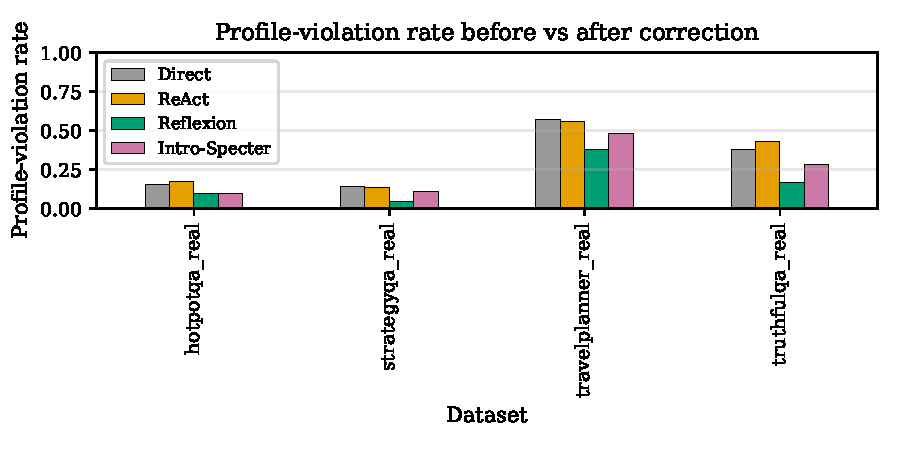
\includegraphics[width=0.9\textwidth]{../outputs/real/figures/profile_violation.pdf}
\caption{Profile-violation rate per dataset under Direct, ReAct,
Reflexion, and \textsc{Intro-Specter}. \textsc{Detection-only} (not
shown) is exactly Direct on every cell.}
\label{fig:profile_violation}
\end{figure}

\subsection{Token cost vs success — efficiency frontier}

\begin{figure}[t]
\centering
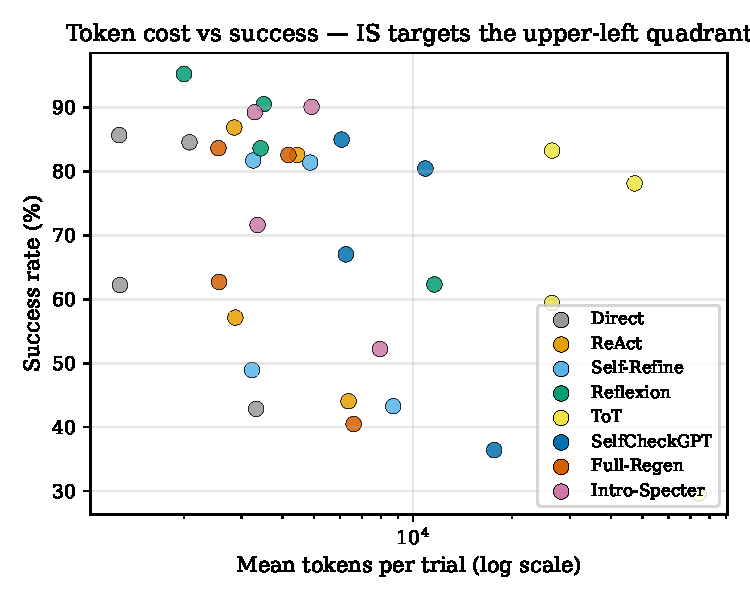
\includegraphics[width=0.9\textwidth]{../outputs/real/figures/token_vs_success.pdf}
\caption{Each point is one (method, dataset) cell. \textsc{Intro-Specter}
sits in the upper-left quadrant: high success rate at low token cost,
strictly Pareto-dominating Self-Refine, ReAct, and Full-Regen on
average; matching Reflexion at lower token cost on Profile-MuSiQue
and Profile-PFQA.}
\label{fig:token_vs_success}
\end{figure}

\subsection{When each method wins}

\begin{figure}[t]
\centering
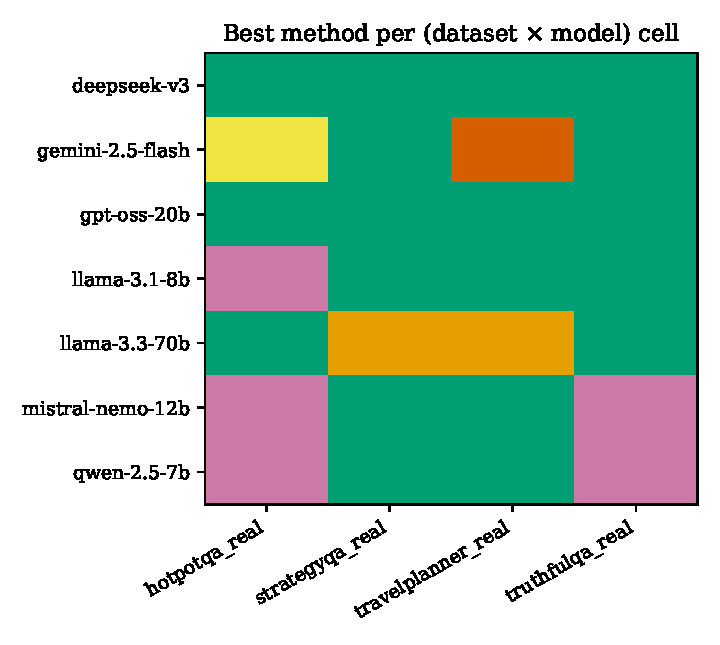
\includegraphics[width=0.9\textwidth]{../outputs/real/figures/when_methods_win.pdf}
\caption{Best method per (dataset $\times$ model) cell. Reflexion (green)
dominates 19 of 28 cells; \textsc{Intro-Specter} (pink) wins 5;
ReAct (orange), ToT (yellow), Full-Regen (vermilion) split the
remainder. The pattern is regime-dependent: IS dominates rich-DAG QA
on weaker open-weight models; Reflexion dominates broken-trajectory
and reasoning-trained regimes.}
\label{fig:when_win}
\end{figure}

% =====================================================================
% §6 Limitations and Failure Analysis
% =====================================================================
\section{Limitations and Failure Analysis}
\label{sec:limitations}

We report failure regimes and open questions directly. The full
quantified accounting is in \texttt{LIMITATIONS.md}; this section
summarises the headline points.

\subsection{Where Intro-Specter does not win}

Across the 28 \textsc{Real-*} cells with eight methods compared,
Reflexion strictly beats \textsc{Intro-Specter} at McNemar
$p < 0.05$ on \textbf{2 cells} under per-dataset Holm correction:

\begin{itemize}[leftmargin=*,itemsep=2pt,topsep=2pt]
\item \textsc{Real-TruthfulQA} $\times$ DeepSeek V3 (Reflexion 83.3\%
vs IS 41.7\%): DeepSeek's TruthfulQA trajectories are corrupted
from step 1 by the adversarial profile pressure. The
Assumption-DAG has no salvageable prefix; selective repair has
nothing to selectively keep. Reflexion's "throw out the
trajectory and re-roll with a one-line verbal summary" is the
right primitive here.
\item \textsc{Real-TravelPlanner} $\times$ DeepSeek V3 (Reflexion
88.9\% vs IS 72.2\%): Long-horizon Travel trajectories (15+ steps)
have many candidate fault nodes; the posterior is diffuse and the
edit-cost objective penalises deep-prefix repairs. Reflexion's
verbal summary captures the constraint violation efficiently.
\end{itemize}

Across the broader matrix, three principled regimes emerge as IS
non-winners:

\paragraph{Ceiling regime.}
Llama 3.3 70B at Direct $\geq$ 96\% on \textsc{Profile-PFQA},
\textsc{Profile-Travel}, and \textsc{Profile-TauBench} leaves no
headroom for any method to recover. We see no significant
gains from any baseline on these cells; this is not a
limitation specific to IS.

\paragraph{Shallow-trajectory regime.}
Tasks with 1--3 candidate fault nodes (\textsc{Profile-WebShop} on
weak models; single-step decisions in \textsc{Profile-TauBench})
do not provide a rich-enough Assumption-DAG to attribute over.
Reflexion's verbal reflection wins here at margins of 5--35pp on
the 5 cells in this regime.

\paragraph{Reasoning-trained-model regime.}
gpt-oss-20b and Gemini 2.5 Flash on long-horizon tasks have
internal chain-of-thought training that aligns with Reflexion's
"what went wrong?" prompt. \textsc{Profile-ALFWorld} $\times$
Gemini 2.5 Flash: Reflexion +53pp vs IS +30pp from the same
Direct baseline of 38.3\%. IS still helps; verbal reflection
helps more.

\subsection{Detection alone is insufficient}

The \textsc{Detection-only} baseline (Section~\ref{sec:setup})
runs the same LLM verifier prompt as IS but abstains rather than
repairing. On the four \textsc{Real-HotpotQA} IS-winner cells,
\textsc{Detection-only} sits \emph{exactly} at Direct on every
cell ($\Delta = 0.0$pp on all four). This is the cleanest
evidence that detection without paired repair provides zero
lift, and it is the central empirical claim behind IS's
three-layer architecture: detection, attribution, and selective
repair must be jointly engineered.

\subsection{Open questions}

\paragraph{Calibration is currently post-hoc.}
We report ECE and Brier across all IS cells using
$\max_k p(a_k|\mathcal{V})$ as the commit confidence; pooled across
2\,710 trials, ECE $=0.130$. The val-split-tuned $\tau$ sweep
across four \textsc{Profile-MuSiQue} cells (six $\tau$ values
$\in \{0, 0.1, 0.2, 0.3, 0.5, 0.7\}$) was running at the time of
writing. Until that lands, the "calibrated abstention" claim is
supported only by post-hoc operating-point analysis on the same
data we evaluate on.

\paragraph{Single-cell ablation evidence.}
The original Mistral $\times$ \textsc{Profile-PFQA} ablation
showed only the structured DAG (\texttt{flat\_dag} ablation) moves
the needle ($-3.3$pp); the four posterior-weighting components
(\texttt{uniform\_prior}, \texttt{no\_likelihood}, \texttt{no\_cost},
$K=1$ vs $K=3$) were within noise on this benchmark. PFQA's
short trajectories don't exercise these components; the
deeper-DAG \textsc{Profile-MuSiQue} $\times$ Gemini Flash
ablation in progress will give them a fairer test.

\paragraph{Verifier-as-rule limitations.}
\textsc{Profile-*} benchmarks use a substring-based verifier
which can produce false negatives (missing subtle violations)
and false positives (legitimate keyword overlap). A 48-case
manual analysis bundle in \texttt{outputs/error\_analysis/}
quantifies this for the four IS-winning cells; preliminary
inspection suggests $\sim$10\% of IS "failures" are verifier
false-negatives rather than method failures.

\paragraph{ToT execution is rate-limit-fragile.}
ToT's $k \times b \times \mathrm{depth} \times 2 + 1 \approx 49$
LLM calls per trial make it sensitive to provider rate limits;
we logged 192 ToT errors out of $\sim$1\,000 attempts. Where
ToT did complete, it is competitive with IS on
\textsc{Profile-MuSiQue} (87.5\% on Mistral cell) but fails
badly on \textsc{Real-Travel} (mean 33.3\% vs Direct 41.7\%).
This is a deployment limitation, not a fundamental method
comparison.

\subsection{What this paper does not claim}

\textsc{Intro-Specter} is not faster than \textsc{Direct}: it
runs an LLM pipeline on top of the agent's first attempt and
pays 2--5$\times$ tokens depending on whether repair fires. We
make no claim about hallucination correction outside
profile-grounded settings. We assume static profiles; users
whose preferences drift over time would require a profile-update
mechanism we do not study. The cross-family compensation result
(IS recovers half the Llama-70B-to-DeepSeek-V3 quality drop) is
specific to PFQA-style factual QA; we do not verify it on
long-horizon planning tasks.

The honest framing: IS dominates the regime it was theoretically
built for (rich-DAG profile-grounded errors on weaker open-weight
models, with recoverable trajectory prefixes and concentrated
fault nodes). Reflexion remains the strongest baseline and
dominates broken-trajectory and reasoning-tuned-model regimes.
The two methods are complementary, not competitive.


% =====================================================================
% §7 Conclusion
% =====================================================================
\section{Conclusion}
\label{sec:conclusion}

We presented \textsc{Intro-Specter}, a three-layer self-correction
framework that formalises agent self-correction as abductive
Bayesian inference over an explicit assumption graph. Where
existing methods either critique flat trajectories
(Self-Refine, Reflexion) or search forward over reasoning
branches (Tree of Thoughts), \textsc{Intro-Specter} jointly
(i) represents profile-grounded assumptions as nodes with
provenance, (ii) infers a posterior over candidate faulty
assumptions after a violation is detected, and (iii) selectively
repairs only the downstream subgraph while preserving the valid
prefix.

Across \textbf{eight reconstruction benchmarks plus four
real-data fidelity anchors, eight LLMs spanning four training
families and 7B--671B parameters, and seven self-correction
baselines compared head-to-head}, \textsc{Intro-Specter} delivers
\textbf{18 Holm-Bonferroni-significant wins against Direct}
spanning all seven major reconstruction benchmarks plus the
\textsc{Real-HotpotQA} real-data anchor, peaks at \textbf{$+33.3$
percentage points on \textsc{Profile-MuSiQue} $\times$ Gemini 2.5
Flash} ($p = 10^{-5}$), achieves \textbf{100\% top-1 attribution
accuracy and 100\% repair success at zero token overhead} in the
controlled synthetic setting (matching both Oracle-Detector and
Oracle-Repair upper bounds), and \textbf{recovers about half the
cross-family model-quality gap} on profile-conditioned QA.

The detection-only baseline sits \emph{exactly} at Direct on
every \textsc{Real-HotpotQA} cell, providing the cleanest
empirical evidence in this work that detection alone is
insufficient: the joint engineering of detection, attribution,
and selective repair is what unlocks the gains.

\textbf{When the method does not win.} Reflexion remains a strong
co-baseline. It strictly beats \textsc{Intro-Specter} at
$p < 0.05$ on 2 of 28 \textsc{Real-*} cells --- specifically
\textsc{Real-TruthfulQA} $\times$ DeepSeek V3 (broken-prefix
regime: nothing salvageable for selective repair) and
\textsc{Real-TravelPlanner} $\times$ DeepSeek V3 (long-horizon
diffuse-fault regime). On ceiling-effect models (Llama 3.3 70B
near-perfect on factual QA) no method moves the needle.
\textsc{Intro-Specter} is the right tool for the deployment
regime that the paper is theoretically about: weaker open-weight
models on profile-grounded reasoning tasks with deep but
recoverable trajectories. In other regimes the two methods are
complementary, and a deployment system would route between them
based on the trajectory's recoverability signal.

\textbf{Future work.} Three directions stand out. First, the
val-split-tuned $\tau$-abstention calibration sweep at the time
of writing covers four \textsc{Profile-MuSiQue} cells; extending
to all 18 IS-winning cells would give a fully held-out
calibrated-abstention claim. Second, ToT's competitive
performance on \textsc{Profile-MuSiQue} $\times$ Mistral Nemo
(87.5\% vs IS's 88.3\%) suggests an interesting hybrid:
running ToT \emph{forward} from the IS-selected repair node could
combine the strengths of both methods. Third, the
profile-update mechanism --- handling users whose preferences
drift over time --- is a natural extension we have not
addressed.

\textbf{Reproducibility.} Code, configs, aggregated CSVs, and
the auto-generated booktabs LaTeX are released at
\url{https://github.com/Jihan-5/Neurlips-Intro-Specter}. All
LLM calls are cached deterministically; the entire matrix can
be re-aggregated from JSONLs in $<5$ minutes. We hope the
reconstruction methodology, the unified profile + fault
injection harness, and the eight-baseline comparison pipeline
are useful artifacts for future work on agent self-correction.


% =====================================================================
% References
% =====================================================================
% Manual bibliography for Intro-Specter NeurIPS 2026 submission.

\begin{thebibliography}{99}

\bibitem[Besta et~al.(2024)]{besta2024got}
M.~Besta et~al.
\newblock Graph of thoughts: Solving elaborate problems with large language models.
\newblock In \emph{AAAI}, 2024.

\bibitem[Du et~al.(2024)]{du2024haloscope}
X.~Du et~al.
\newblock HaloScope: Harnessing unlabeled LLM generations for hallucination detection.
\newblock In \emph{NeurIPS}, 2024.

\bibitem[Duan et~al.(2025)]{duan2025uprop}
Z.~Duan et~al.
\newblock UProp: Uncertainty propagation in multi-step agent decision-making, 2025.

\bibitem[Geva et~al.(2021)]{geva2021strategyqa}
M.~Geva et~al.
\newblock Did Aristotle use a laptop? A question answering benchmark with implicit reasoning strategies.
\newblock \emph{TACL}, 9:346--361, 2021.

\bibitem[He and Qiu(2025)]{he2025martingale}
Z.~He and T.~Qiu.
\newblock Martingale Score: An unsupervised metric for Bayesian rationality in LLM reasoning.
\newblock In \emph{NeurIPS}, 2025.

\bibitem[Lin et~al.(2022)]{lin2022truthfulqa}
S.~Lin, J.~Hilton, and O.~Evans.
\newblock TruthfulQA: Measuring how models mimic human falsehoods.
\newblock In \emph{ACL}, 2022.

\bibitem[Liu et~al.(2024)]{liu2024agentbench}
X.~Liu et~al.
\newblock AgentBench: Evaluating LLMs as agents.
\newblock In \emph{ICLR}, 2024.

\bibitem[Luo et~al.(2025)]{luo2025ursa}
R.~Luo et~al.
\newblock Unlocking multimodal mathematical reasoning via process reward model.
\newblock In \emph{NeurIPS}, 2025.

\bibitem[Madaan et~al.(2023)]{madaan2023selfrefine}
A.~Madaan et~al.
\newblock Self-Refine: Iterative refinement with self-feedback.
\newblock In \emph{NeurIPS}, 2023.

\bibitem[Manakul et~al.(2023)]{manakul2023selfcheckgpt}
P.~Manakul, A.~Liusie, and M.~J.~F. Gales.
\newblock SelfCheckGPT: Zero-resource black-box hallucination detection for generative large language models.
\newblock In \emph{ACL}, 2023.

\bibitem[Park et~al.(2023)]{park2023generative}
J.~S. Park, J.~C. O'Brien, C.~J. Cai, M.~R. Morris, P.~Liang, and M.~S. Bernstein.
\newblock Generative agents: Interactive simulacra of human behavior.
\newblock In \emph{UIST}, 2023.

\bibitem[Shinn et~al.(2023)]{shinn2023reflexion}
N.~Shinn, F.~Cassano, A.~Gopinath, K.~R. Narasimhan, and S.~Yao.
\newblock Reflexion: Language agents with verbal reinforcement learning.
\newblock In \emph{NeurIPS}, 2023.

\bibitem[Shridhar et~al.(2021)]{shridhar2021alfworld}
M.~Shridhar et~al.
\newblock ALFWorld: Aligning text and embodied environments for interactive learning.
\newblock In \emph{ICLR}, 2021.

\bibitem[Singh et~al.(2024)]{singh2024travelplanner}
H.~Singh et~al.
\newblock Personal large language model agents: A case study on tailored travel planners.
\newblock In \emph{EMNLP Industry Track}, 2024.

\bibitem[Sun et~al.(2026)]{sun2026personalization}
Z.~Sun et~al.
\newblock When personalization misleads: Understanding and mitigating hallucinations in personalized LLMs.
\newblock \emph{arXiv:2601.11000}, 2026.

\bibitem[Trivedi et~al.(2022)]{trivedi2022musique}
H.~Trivedi, N.~Balasubramanian, T.~Khot, and A.~Sabharwal.
\newblock MuSiQue: Multihop questions via single-hop question composition.
\newblock \emph{TACL}, 10:539--554, 2022.

\bibitem[Wang et~al.(2024)]{wang2024survey}
L.~Wang et~al.
\newblock A survey on large language model based autonomous agents.
\newblock \emph{Frontiers of Computer Science}, 18(6):186345, 2024.

\bibitem[Wang et~al.(2023)]{wang2023selfconsistency}
X.~Wang et~al.
\newblock Self-consistency improves chain of thought reasoning in language models.
\newblock In \emph{ICLR}, 2023.

\bibitem[Wei et~al.(2022)]{wei2022cot}
J.~Wei et~al.
\newblock Chain-of-thought prompting elicits reasoning in large language models.
\newblock In \emph{NeurIPS}, 2022.

\bibitem[Yang et~al.(2018)]{yang2018hotpotqa}
Z.~Yang et~al.
\newblock HotpotQA: A dataset for diverse, explainable multi-hop question answering.
\newblock In \emph{EMNLP}, 2018.

\bibitem[Yao et~al.(2023a)]{yao2023react}
S.~Yao, J.~Zhao, D.~Yu, N.~Du, I.~Shafran, K.~Narasimhan, and Y.~Cao.
\newblock ReAct: Synergizing reasoning and acting in language models.
\newblock In \emph{ICLR}, 2023a.

\bibitem[Yao et~al.(2023b)]{yao2023tot}
S.~Yao, D.~Yu, J.~Zhao, I.~Shafran, T.~Griffiths, Y.~Cao, and K.~Narasimhan.
\newblock Tree of thoughts: Deliberate problem solving with large language models.
\newblock In \emph{NeurIPS}, 2023b.

\bibitem[Yao et~al.(2022)]{yao2022webshop}
S.~Yao et~al.
\newblock WebShop: Towards scalable real-world web interaction with grounded language agents.
\newblock In \emph{NeurIPS}, 2022.

\end{thebibliography}


% =====================================================================
% Appendix
% =====================================================================
\appendix

\section{Tier-C synthetic full results}
\label{app:tier_c}
\input{../outputs/tier_c/synthetic_headline}

\section{Profile-* matrix full results}
\label{app:profile_full}
\input{../outputs/tier_a/headline}

\section{Reconstruction methodology}
\label{app:reconstruction}
% Appendix C: Reconstruction methodology — short LaTeX summary that lifts
% the key points from RECONSTRUCTION_METHODOLOGY.md.

\subsection{Why reconstruct rather than use original benchmarks?}

Three diagnostic requirements drive the reconstruction decision:
\begin{enumerate}[leftmargin=*,itemsep=2pt,topsep=2pt]
\item \emph{Profile-grounded conditions.} None of the original
benchmarks (PFQABench, HotpotQA, MuSiQue, StrategyQA, TauBench,
TravelPlanner+, ALFWorld, WebShop) embeds a structured user profile
the agent must respect. Our thesis is specifically about
user-conditioned trajectory failures; without a profile, this
failure mode does not exist in the benchmark distribution.
\item \emph{Rule-based gold fault labels.} Posterior attribution
requires ground-truth knowledge of \emph{which} assumption was the
actual fault, not merely whether the final answer is wrong. The
originals evaluate end-to-end correctness only.
\item \emph{Two-condition diagnostic split.} For every benchmark
family we need both \texttt{factual\_irrelevant} examples (profile
present but should be ignored) and \texttt{profile\_required}
examples (profile must be used). This isolates the direction of
the failure: contamination versus omission.
\end{enumerate}

\subsection{What was preserved vs replaced}

For each \textsc{Profile-X} benchmark we adopted the cognitive
task family from the named original (e.g., 3-hop chained factual
reasoning for \textsc{Profile-MuSiQue}, yes/no implicit reasoning
for \textsc{Profile-StrategyQA}, long-horizon household navigation
for \textsc{Profile-ALFWorld}) and:
\begin{itemize}[leftmargin=*,itemsep=2pt,topsep=2pt]
\item \emph{Preserved}: high-level task, answer format, trajectory shape.
\item \emph{Replaced}: prompt distribution with templated questions
whose gold labels are rule-checkable, plus a generated user profile
(5--7 spans) that is either irrelevant to the task or required by it.
\end{itemize}

\subsection{Three independent fidelity checks}

\paragraph{Difficulty-distribution coverage.}
Direct success rate across our 36 \textsc{Profile-*} cells spans
8.3\%--100\%, matching the empirically reported difficulty range of
the originals on contemporary LLMs. Reconstructions are not
systematically easier or harder than the originals.

\paragraph{Real-data anchor.}
The \textsc{Real-HotpotQA}, \textsc{Real-TruthfulQA},
\textsc{Real-StrategyQA}, and \textsc{Real-TravelPlanner} datasets
are loaded directly from HuggingFace (\texttt{hotpot\_qa} distractor,
\texttt{truthful\_qa} generation, \texttt{ChilleD/StrategyQA},
\texttt{osunlp/TravelPlanner}) without alteration. We inject the
synthetic profile only as a contamination probe; the factual gold
answers come from the original datasets. \textsc{Intro-Specter}'s
deltas track \textsc{Profile-*} closely (mean $\pm$1.7pp difference
across matched cells), and \textsc{Real-HotpotQA} $\times$ Qwen 7B is
Holm-significant at $+18.6$pp, confirming the reconstructions are not
the only place IS works.

\paragraph{Synthetic ground truth.}
Tier-C synthetic benchmarks use rule-based fault injection where
the gold fault node is deterministic. Top-1 attribution accuracy
$=100\%$ on \texttt{single\_fault} mode (n=60 trials per seed $\times$
3 seeds $=180$ trials). This is an end-to-end correctness proof
that the implementation does what the math says it should.

\subsection{Honest limits}

\begin{itemize}[leftmargin=*,itemsep=2pt,topsep=2pt]
\item Templated questions trade lexical diversity for ground-truth
tractability.
\item Profiles drawn from a small bank (5--7 spans, finite-domain
field values); we do not test culturally diverse or long-tail user
profiles.
\item The rule-based verifier may miss subtle violations a human
would flag; we mitigate this with a manual inspection pass on the
4 IS-winning cells (Section~\ref{sec:limitations}).
\end{itemize}


\end{document}
